%\documentclass[compress]{beamer}
\documentclass[handout]{beamer}

\usepackage[T1]{fontenc}
\usepackage[american]{babel}
\usepackage{csquotes}
\usepackage[style=apa, backend=biber]{biblatex}
\usepackage{pifont}
\usepackage{threeparttable}
\usepackage{subcaption}
\usepackage{tikz-qtree}
\usepackage{tikz}
\usepackage{multicol}
\usepackage{booktabs}
\usepackage{graphicx}
\usepackage{neuralnetwork}
\usepackage{hyperref}
\usepackage{fancyvrb}
\usepackage{xcolor}
\usepackage{minted}


\addbibresource{../literature.bib}
\graphicspath{{../resources/pictures/}}

\hypersetup{
  pdfborder={0 0 0},
  colorlinks=true,
  pdfauthor={Anne Kroon, Saurabh Khanna},
  pdftitle={Computational Communication Science 2}
}

\usetheme[block=fill,subsectionpage=progressbar,sectionpage=progressbar]{metropolis}
\definecolor{Purple}{HTML}{911146}
\definecolor{Orange}{HTML}{CF4A30}
\setbeamercolor{alerted text}{fg=Orange}
\setbeamercolor{frametitle}{bg=Purple,fg=white}
\setbeamercolor{structure}{fg=Purple}
\setbeamercolor{normal text}{bg=white,fg=black}
\setbeamercovered{still covered={\opaqueness<1->{5}},again covered={\opaqueness<1->{100}}}
\setbeamersize{text margin left=12pt,text margin right=12pt}
\setbeamertemplate{section page}[progressbar]
\setbeamertemplate{subsection page}[progressbar]
\setbeamertemplate{itemize item}{\color{Purple}$\bullet$}
\setbeamerfont{frametitle}{size=\Large,series=\bfseries}
\setbeamerfont{framesubtitle}{size=\normalsize}
\setbeamerfont{normal text}{size=\small}
\setbeamerfont{itemize/enumerate body}{size=\small}
\setbeamerfont{itemize/enumerate subbody}{size=\small}
\setbeamerfont{block title}{size=\large,series=\bfseries}
\renewcommand*{\bibfont}{\tiny}

\makeatletter
\setbeamertemplate{headline}{%
    \begin{beamercolorbox}[colsep=1.5pt]{upper separation line head}
    \end{beamercolorbox}
    \begin{beamercolorbox}{section in head/foot}
        \vskip2pt\insertnavigation{\paperwidth}\vskip2pt
    \end{beamercolorbox}%
    \begin{beamercolorbox}[colsep=1.5pt]{lower separation line head}
    \end{beamercolorbox}
}
\makeatother

\usemintedstyle{colorful}
\setminted{breaklines, fontsize=\tiny, bgcolor=gray!5}

\newcommand{\question}[1]{
    \begin{frame}[plain]
        \begin{columns}
            \column{.4\textwidth}
            \makebox[\columnwidth]{%
                
\includegraphics[width=\columnwidth,height=\paperheight,keepaspectratio]{mannetje.png}}
            \column{.6\textwidth}
            \large
            \textcolor{Orange}{\textbf{\emph{#1}}}
        \end{columns}
    \end{frame}
}
\newcommand{\instruction}[1]{\emph{\textcolor{gray}{[#1]}}}

\title[CCS2]{\textbf{Computational Communication Science 2} \\
Week 2 -- Lecture\\
\emph{Text Representation: Preprocessing, Vectorizers, and Embeddings}}
\author[Anne Kroon]{Anne Kroon \\ \footnotesize{a.c.kroon@uva.nl}}
\date{April 7, 2026}
\institute[Digital Society Minor]{Digital Society Minor, University of Amsterdam}

\begin{document}

\begin{frame}{}
    \titlepage
\end{frame}

\begin{frame}{Today's Agenda}
    \begin{tiny}\tableofcontents\end{tiny}
\end{frame}

% ================================
\section{Recap}
% ================================

\begin{frame}{Review of Key Concepts}
    \begin{itemize}
        \item \textbf{Text as data:} digital communication produces large amounts of text
        \item \textbf{Two approaches:}
        \begin{itemize}
            \item \emph{Bottom-up}: explore patterns without predefined categories
            \item \emph{Top-down}: measure predefined concepts
        \end{itemize}
        \item \textbf{Preprocessing:} cleaning and preparing raw text
        \begin{itemize}
            \item Tokenization, stopword removal, basic string methods
        \end{itemize}
    \end{itemize}
    \vspace{0.3cm}
    Today we go deeper into preprocessing and move on to text representation.
\end{frame}

% ================================
\section{Preprocessing in depth}
% ================================

\subsection{Tokenization}

\begin{frame}[fragile]{Tokenization: a reminder}
\textbf{Goal:} split a string into a list of tokens.

\begin{minted}{python}
from nltk.tokenize import TreebankWordTokenizer

docs = ["Communication in the digital society is very complex",
        "I like to study it"]

tokens = [TreebankWordTokenizer().tokenize(d) for d in docs]
print(tokens)
\end{minted}

\pause

\begin{minted}{text}
[['Communication', 'in', 'the', 'digital', 'society',
  'is', 'very', 'complex'],
 ['I', 'like', 'to', 'study', 'it']]
\end{minted}

\textbf{Result:} one list of tokens per document.
\end{frame}

\begin{frame}{What is a token?}
A \textbf{token} is the basic unit of analysis after splitting text.

\vspace{0.5em}
Tokens are usually single words, but can also be sequences of words:

\vspace{0.5em}
\begin{tabular}{lll}
    \textbf{Type} & \textbf{n} & \textbf{Example} \\
    \midrule
    Unigram & 1 & \texttt{"digital"}, \texttt{"society"} \\
    Bigram  & 2 & \texttt{"digital society"} \\
    Trigram & 3 & \texttt{"the digital society"} \\
\end{tabular}

\vspace{0.5em}
\textbf{Why multi-word tokens?} Single words sometimes lose important context.\\
\emph{"not good"} means something very different from \emph{"good"}.

\vspace{0.3em}
\small In scikit-learn, set \texttt{ngram\_range=(1,2)} in \texttt{CountVectorizer} to include both unigrams and bigrams.
\end{frame}

\subsection{Stemming and lemmatization}

\begin{frame}{Stemming vs.\ lemmatization}
Both reduce token forms to a common base --- but differently.

\vspace{0.5em}
\begin{columns}
\column{0.5\textwidth}
\begin{block}{Stemming}
\begin{itemize}
    \item Chops off endings using rules
    \item Fast, but can produce non-words
    \item \texttt{"society"} $\to$ \texttt{"societi"}
\end{itemize}
\end{block}
\column{0.5\textwidth}
\begin{block}{Lemmatization}
\begin{itemize}
    \item Maps to dictionary form
    \item Slower, but linguistically accurate
    \item \texttt{"better"} $\to$ \texttt{"good"}
\end{itemize}
\end{block}
\end{columns}
\end{frame}

\begin{frame}[fragile]{Stemming in practice}
\textbf{Note:} stemming is applied \emph{per token} --- loop over documents \emph{and} tokens.

\begin{minted}{python}
from nltk.stem import PorterStemmer

stemmer = PorterStemmer()

# tokens is a list of lists
tokens_stemmed = [[stemmer.stem(token) for token in doc]
                  for doc in tokens]
print(tokens_stemmed)
\end{minted}

\pause

\begin{minted}{text}
[['commun', 'in', 'the', 'digit', 'societi', 'is', 'veri', 'complex'],
 ['i', 'like', 'to', 'studi', 'it']]
\end{minted}

\pause
\small Stemming can produce non-standard forms (\texttt{societi}, \texttt{veri}) --- this is expected. Stemming is a heuristic, not a dictionary lookup.
\end{frame}

\begin{frame}[fragile]{Lemmatization in practice: NLTK}
Like stemming, lemmatization is applied \emph{per token}.\\
With NLTK's \texttt{WordNetLemmatizer}, the default assumes every token is a \textbf{noun}:

\begin{minted}{python}
from nltk.stem import WordNetLemmatizer

lemmatizer = WordNetLemmatizer()

words = ["studies", "geese", "running", "better"]
print([lemmatizer.lemmatize(w) for w in words])
\end{minted}

\pause

\begin{minted}{text}
['study', 'goose', 'running', 'better']
\end{minted}

\pause
\small \textbf{Problem:} \texttt{"running"} and \texttt{"better"} are not reduced --- the lemmatizer does not know they are a verb and adjective. Fixing this requires providing POS tags manually, which is impractical at scale.
\end{frame}

\begin{frame}[fragile]{Lemmatization in practice: spaCy}
\textbf{spaCy} handles POS tagging \emph{automatically} --- no manual tags needed.

\begin{minted}{python}
import spacy
nlp = spacy.load("en_core_web_sm")

doc = nlp("The studies show that running is better than doing nothing")
# show only tokens where lemma differs from the original
print([(t.text, t.lemma_) for t in doc if t.text != t.lemma_])
\end{minted}

\pause

\begin{minted}{text}
[('studies', 'study'), ('running', 'run'),
 ('is', 'be'), ('better', 'good'), ('doing', 'do')]
\end{minted}

\pause
\small \texttt{"running"} $\to$ \texttt{"run"}, \texttt{"better"} $\to$ \texttt{"good"}, \texttt{"studies"} $\to$ \texttt{"study"} --- all correct, automatically.
\end{frame}

% ================================
\section{Building text representations: vectorizers}
% ================================

\subsection{From text to vectors}

\begin{frame}[fragile]{A text as a bag of words}
The simplest representation: count how often each token appears.

\begin{minted}{python}
from collections import Counter

t = "This this is is is a test test test"
print(Counter(t.split()))
\end{minted}

\begin{minted}{text}
Counter({'is': 3, 'test': 3, 'This': 1, 'this': 1, 'a': 1})
\end{minted}

\pause
This representation:
\begin{itemize}
    \item preserves token frequencies
    \item does \emph{not} preserve word order
    \item can be treated as a \textbf{vector} we can calculate with
\end{itemize}

\small \emph{Note: \texttt{This} and \texttt{this} are counted separately --- lowercasing matters!}
\end{frame}

\begin{frame}{From vectors to a matrix}
Stacking one vector per document gives a \textbf{document-term matrix (DTM)}.

\vspace{0.5em}
\texttt{t1 = "This this is is is a test test test"}\\
\texttt{t2 = "This is an example"}

\vspace{0.5em}
\begin{tabular}{|l|c|c|c|c|c|c|c|}
    \hline
    & \texttt{a} & \texttt{an} & \texttt{example} & \texttt{is} & \texttt{This} & \texttt{this} & \texttt{test} \\
    \hline
    \emph{t1} & 1 & 0 & 0 & 3 & 1 & 1 & 3 \\
    \emph{t2} & 0 & 1 & 1 & 1 & 1 & 0 & 0 \\
    \hline
\end{tabular}

\vspace{0.5em}
\small Each row = document; each column = token; each cell = count.\\
\textbf{Note:} \texttt{This} and \texttt{this} are separate columns --- treated as different tokens without lowercasing!
\end{frame}

\question{What can you do with such a matrix? Why represent texts this way?}

\begin{frame}{What is a vectorizer?}
    \begin{itemize}[<+->]
        \item Automates building a DTM from raw text
        \item First \textbf{fitted} on a corpus: learns which \textbf{tokens} exist and assigns them to columns
        \item Can then \textbf{transform} new texts into the same feature space
        \item Result: a \textbf{sparse matrix} --- only non-zero values stored
    \end{itemize}
\end{frame}

\begin{frame}[fragile]{CountVectorizer: basic usage}
\begin{minted}{python}
from sklearn.feature_extraction.text import CountVectorizer

docs = ["Communication in the digital society is very complex",
        "I like to study it"]

cv = CountVectorizer()
dtm = cv.fit_transform(docs)

print(cv.get_feature_names_out())
print(dtm.toarray())
\end{minted}

\pause

\begin{minted}{text}
['communication' 'complex' 'digital' 'in' 'is' 'it'
 'like' 'society' 'study' 'the' 'to' 'very']

[[1 1 1 1 1 0 0 1 0 1 0 1]
 [0 0 0 0 0 1 1 0 1 0 1 0]]
\end{minted}

\small \textbf{Note:} CountVectorizer lowercases and removes punctuation by default.
\end{frame}

\subsection{Weighting: TF-IDF}

\begin{frame}{Are all tokens equally informative?}
Raw counts treat all tokens the same.

\vspace{0.5em}
\begin{itemize}
    \item \texttt{"the"} appears in almost every document --- tells us very little
    \item \texttt{"misinformation"} in only a few documents --- much more distinctive
\end{itemize}

\vspace{0.5em}
\textbf{Idea:} downweight frequent tokens, upweight rare ones.\\
$\Rightarrow$ This is what \textbf{TF-IDF} does.
\end{frame}

\begin{frame}{TF-IDF: the formula}
\[
\text{tf-idf}_{i,j} = \text{tf}_{i,j} \times \log \left(\frac{N}{\text{df}_i}\right)
\]

\begin{itemize}
    \item $\text{tf}_{i,j}$ = how often token $i$ appears in document $j$
    \item $\text{df}_i$ = number of documents containing token $i$
    \item $N$ = total number of documents
\end{itemize}

\vspace{0.5em}
\textbf{Intuition:}
\begin{itemize}
    \item High TF + low DF $\rightarrow$ high score (important for this doc, rare overall)
    \item High DF $\rightarrow$ low score (common tokens like \texttt{"the"})
\end{itemize}

\small \emph{scikit-learn applies additional normalization --- see documentation.}
\end{frame}

\begin{frame}{TF-IDF vs.\ raw counts}
\begin{columns}
\column{0.5\textwidth}
\begin{block}{Raw counts}
\begin{itemize}
    \item Interpretable
    \item Describes a document on its own
    \item Good when frequency itself matters
\end{itemize}
\end{block}
\column{0.5\textwidth}
\begin{block}{TF-IDF}
\begin{itemize}
    \item Adjusts for common tokens
    \item Better for comparing documents
    \item Good for search and classification
\end{itemize}
\end{block}
\end{columns}

\vspace{0.5em}
\textbf{Bottom line:} it is an empirical question --- try both and evaluate.
\end{frame}

\subsection{Pruning}

\begin{frame}{Pruning: reducing the feature space}
\begin{itemize}
    \item \textbf{Stopword removal:} fixed list, does not adapt to your corpus
    \item \textbf{TF-IDF:} downweights frequent tokens, but keeps them in the matrix
    \item \textbf{Pruning:} removes tokens based on empirical frequency in \emph{your} corpus
\end{itemize}

\vspace{0.5em}
\textbf{Parameters in scikit-learn:}
\begin{itemize}
    \item \texttt{max\_df}: drop tokens appearing in more than X\% of documents
    \item \texttt{min\_df}: drop tokens appearing in fewer than $n$ documents
\end{itemize}
\end{frame}

\begin{frame}[fragile]{Putting it all together}
\textbf{Step 1:} stopwords only
\begin{minted}{python}
cv = CountVectorizer(stop_words=mystopwords)
\end{minted}

\textbf{Step 2:} add a better tokenizer
\begin{minted}{python}
cv = CountVectorizer(
    tokenizer=TreebankWordTokenizer().tokenize,
    stop_words=mystopwords)
\end{minted}

\textbf{Step 3:} add pruning
\begin{minted}{python}
cv = CountVectorizer(
    tokenizer=TreebankWordTokenizer().tokenize,
    stop_words=mystopwords,
    max_df=0.75, min_df=2)
\end{minted}

\textbf{Step 4:} switch to TF-IDF
\begin{minted}{python}
from sklearn.feature_extraction.text import TfidfVectorizer
tfidf = TfidfVectorizer(
    tokenizer=TreebankWordTokenizer().tokenize,
    stop_words=mystopwords,
    max_df=0.75, min_df=2)
\end{minted}
\end{frame}

\question{Which combination is ``best'' --- and how do you decide?}

\begin{frame}{Sparse matrices}
    \begin{block}{Why sparse?}
        \begin{itemize}
            \item A DTM can have tens of thousands of columns (one per token)
            \item Most cells are zero --- storing all of them wastes memory
            \item \textbf{Sparse matrix:} only non-zero values and positions are stored
            \item Never convert to dense / DataFrame on real data!
        \end{itemize}
    \end{block}
\end{frame}

{\setbeamercolor{background canvas}{bg=black}
    \begin{frame}
        \makebox[\linewidth]{
            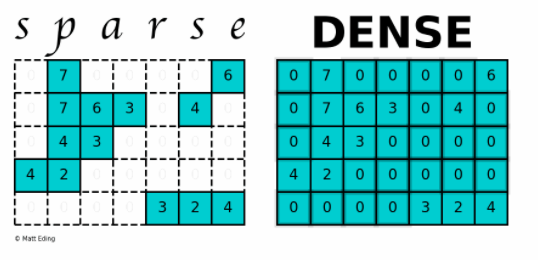
\includegraphics[width=\paperwidth,height=\paperheight,keepaspectratio]{sparse_dense.png}}
        \url{https://matteding.github.io/2019/04/25/sparse-matrices/}
    \end{frame}
}

\begin{frame}{Explore vectorizers interactively}
    \begin{alertblock}{Best of both worlds}
        Use \texttt{CountVectorizer} or \texttt{TfidfVectorizer} with an NLTK-based tokenizer for full control.
    \end{alertblock}
    \vspace{0.5em}
    Try it out yourself:
    \vspace{0.3em}
    \href{https://apps-computational-teaching-jj92xohbgnwnhksxlclr8t.streamlit.app}{DTM Explorer (Streamlit app)}
\end{frame}

\begin{frame}{Go further in code}
    \begin{alertblock}{try it out}
        Use \texttt{CountVectorizer} or \texttt{TfidfVectorizer} with an NLTK-based tokenizer.
    \end{alertblock}
    \vspace{0.5em}
    \href{https://github.com/uva-cw-ccs2/2526s2/blob/main/week02/exercise-lecture/Understanding_vectorizers.ipynb}{Notebook: Understanding vectorizers}\\
    \vspace{0.3em}
    \tiny{\url{https://scikit-learn.org/stable/modules/generated/sklearn.feature\_extraction.text.CountVectorizer.html}}
\end{frame}

% ================================
\section{Introducing embeddings}
% ================================

\begin{frame}{Why should communication scientists care about embeddings?}

    As communication researchers, we often want to know:
    \begin{itemize}
        \item Are these two news articles about the same topic?
        \item How similar is the language used by different politicians?
        \item Does the meaning of a word (e.g., \emph{"populism"}) shift over time?
    \end{itemize}

    \vspace{0.5em}
    \textbf{TF-IDF cannot answer these questions well} --- it treats every token as independent and has no notion of meaning.

    \vspace{0.5em}
    \textbf{Word embeddings} open the door to meaning-aware text analysis.
\end{frame}

\begin{frame}{The problem with bag-of-words}
    Consider these two sentences:
    \begin{itemize}
        \item \emph{"The president gave a speech about climate change."}
        \item \emph{"The leader delivered a talk on global warming."}
    \end{itemize}

    \vspace{0.5em}
    \pause
    To a human, these sentences mean almost the same thing.\\
    To a bag-of-words model, they share \textbf{only one token}: \texttt{"a"}.

    \vspace{0.5em}
    \pause
    \textbf{Why?} Because \texttt{"president"} and \texttt{"leader"}, \texttt{"speech"} and \texttt{"talk"}, \texttt{"climate change"} and \texttt{"global warming"} are treated as completely unrelated.

    \vspace{0.5em}
    We need a representation that captures \textbf{meaning}, not just token identity.
\end{frame}

\begin{frame}{From sparse to dense: the key idea}
    \textbf{Bag-of-words (sparse):} one dimension per token in the vocabulary.

    \vspace{0.3em}
    \texttt{king = [1, 0, 0, 0, 0, 0, ..., 0]}  \hfill (tens of thousands of dimensions)

    \vspace{0.8em}
    \textbf{Word embedding (dense):} a short vector of real numbers.

    \vspace{0.3em}
    \texttt{king = [0.32, $-$0.14, 0.87, 0.05, $-$0.61, ...]}  \hfill (100--300 dimensions)

    \vspace{0.8em}
    \pause
    Each number captures some \textbf{latent aspect of meaning} --- we do not define what each dimension means; the model figures it out from data.

    \vspace{0.5em}
    \small Words used in similar contexts end up with \textbf{similar vectors}.
\end{frame}

\subsection{Word embeddings}

\begin{frame}{How are embeddings learned?}
    \begin{block}{Core idea (Firth, 1957)}
        \emph{``A word is characterized by the company it keeps.''}
    \end{block}

    \vspace{0.5em}
    \begin{itemize}[<+->]
        \item A model is trained on a large corpus (e.g., Wikipedia, news articles)
        \item It learns to \textbf{predict} which words appear near each other
        \item Words that appear in similar contexts get \textbf{similar vectors}
        \item No manual labelling needed --- the signal comes from the text itself
        \item Popular models: \textbf{Word2Vec}, \textbf{GloVe}, \textbf{fastText}
    \end{itemize}
\end{frame}

\begin{frame}{}
    \makebox[\linewidth]{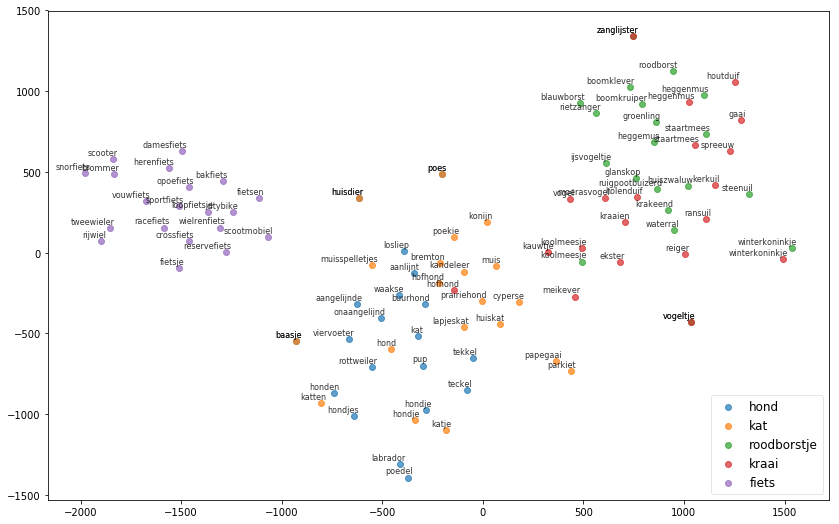
\includegraphics[width=\linewidth,height=\textheight,keepaspectratio]{w2v_300_illustration.png}}
\end{frame}

\begin{frame}{Similar words, similar vectors}
    Because embeddings are learned from context, words with related meanings end up \textbf{close together} in vector space.

    \vspace{0.5em}
    \begin{itemize}
        \item \texttt{"dog"} and \texttt{"cat"} are close --- both are pets
        \item \texttt{"king"} and \texttt{"queen"} are close --- both are royalty
        \item \texttt{"happy"} and \texttt{"joyful"} are close --- synonyms
    \end{itemize}

    \vspace{0.5em}
    \pause
    This also means you can do \textbf{arithmetic} with meaning:
    \[
    \vec{\text{king}} - \vec{\text{man}} + \vec{\text{woman}} \approx \vec{\text{queen}}
    \]

    \small The geometry of the vector space reflects real-world relationships --- something TF-IDF vectors cannot do.
\end{frame}

\begin{frame}{Visualizing word embeddings}
    \begin{columns}
        \column{0.5\textwidth}
        \makebox[\columnwidth]{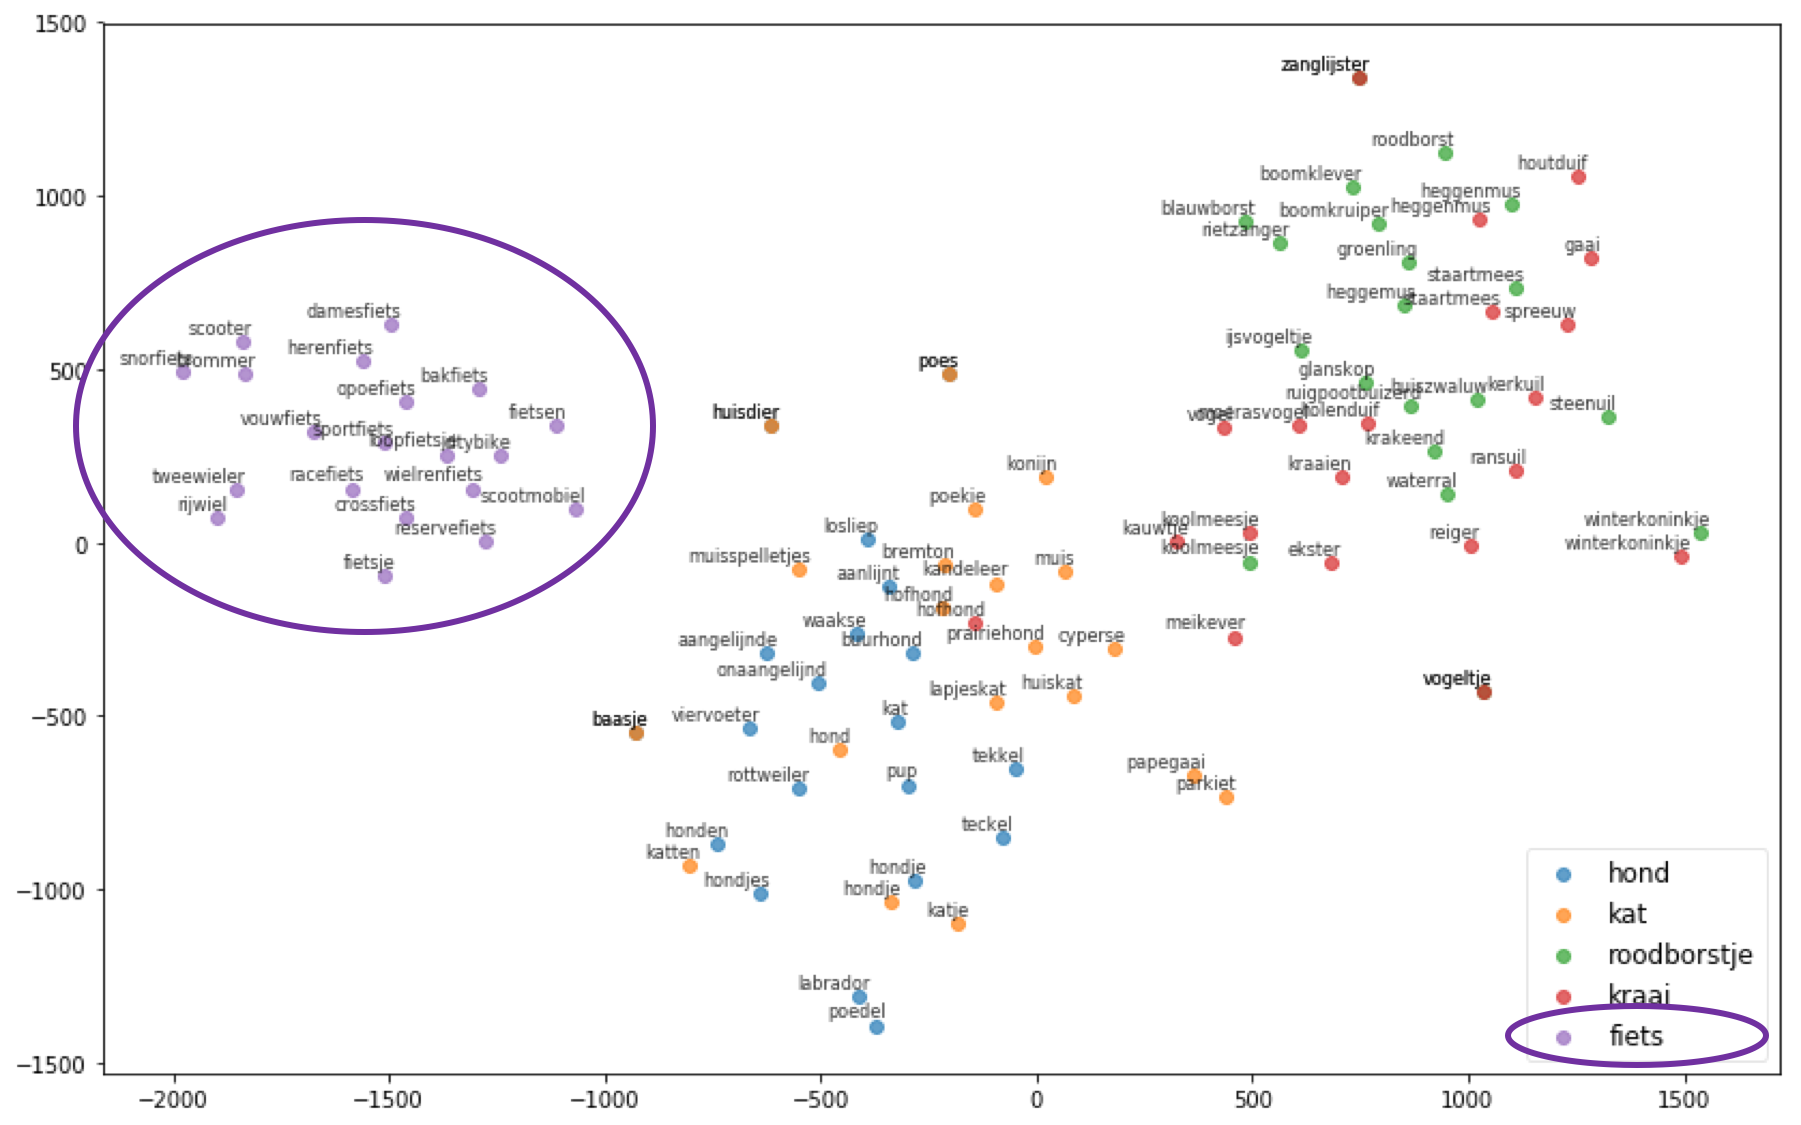
\includegraphics[width=\columnwidth,height=0.7\textheight,keepaspectratio]{visual2.png}}
        \column{0.5\textwidth}
        \makebox[\columnwidth]{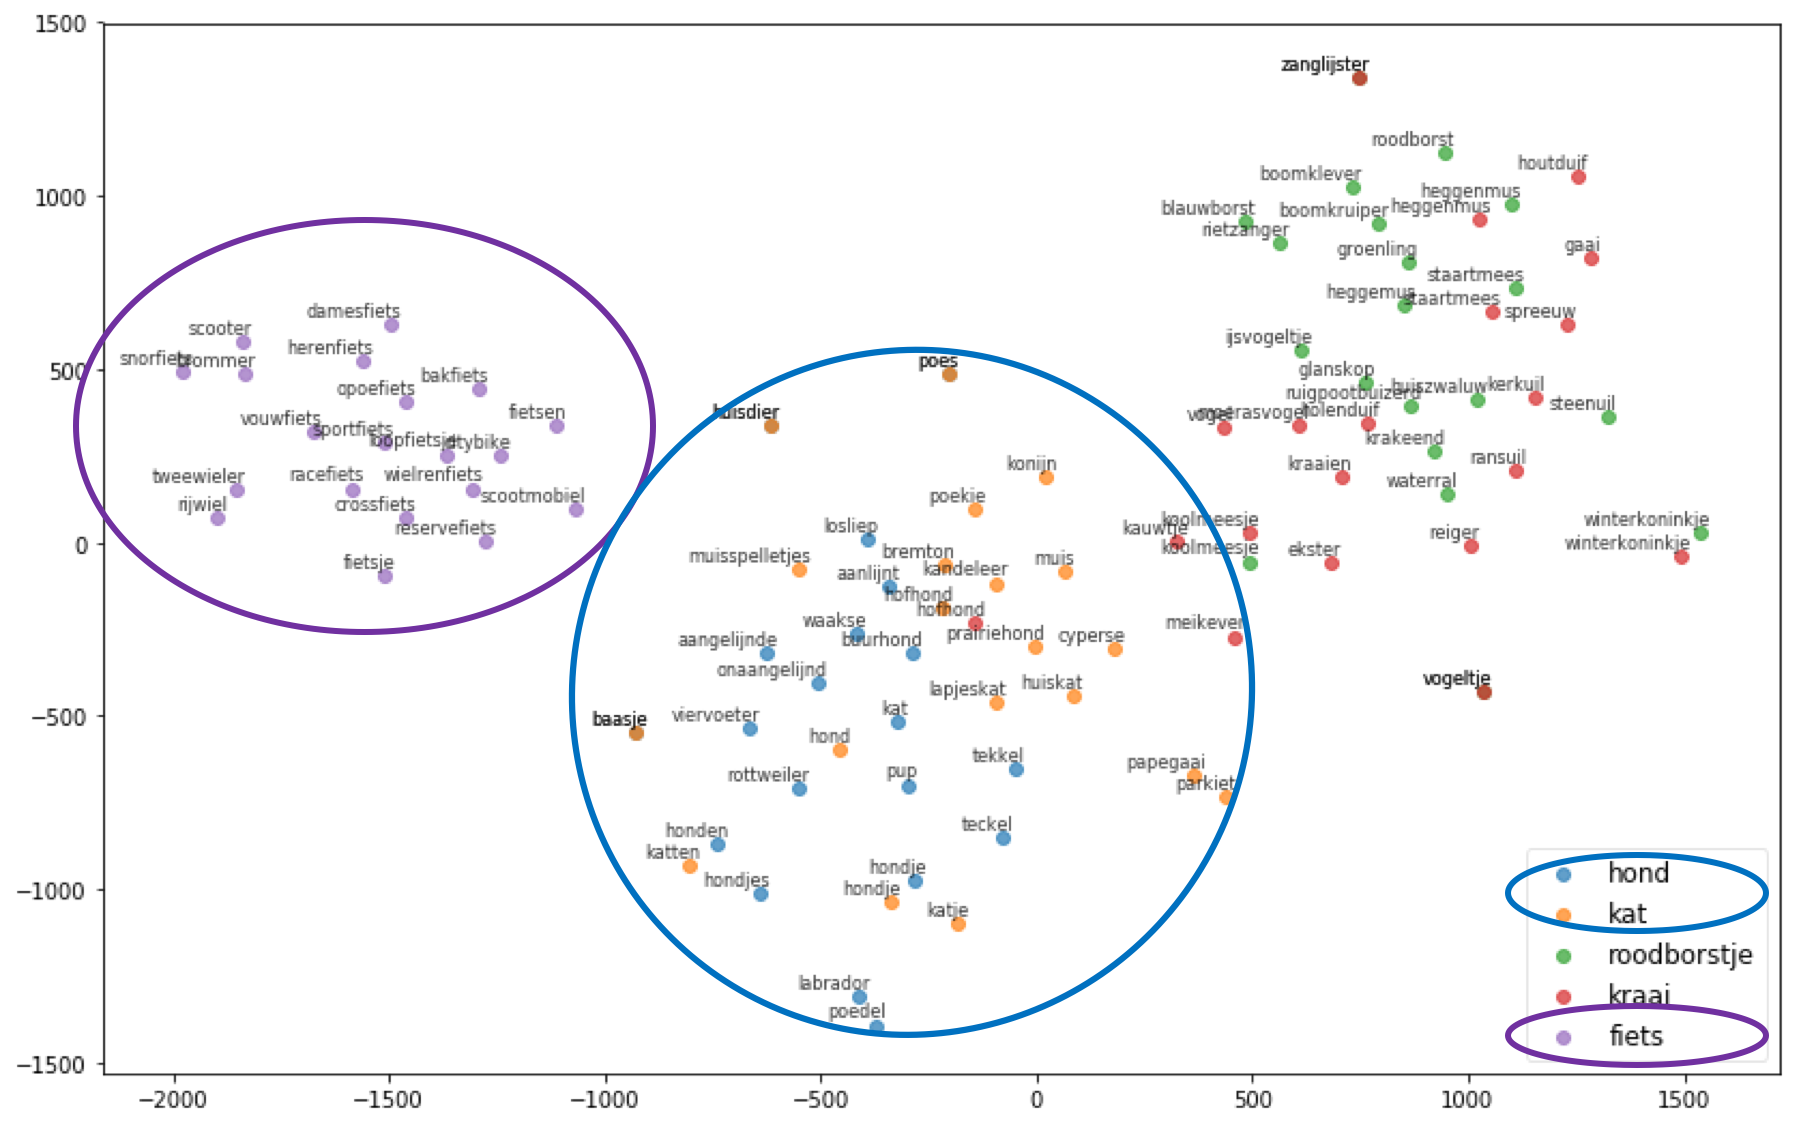
\includegraphics[width=\columnwidth,height=0.7\textheight,keepaspectratio]{visual1.png}}
    \end{columns}
    \vspace{0.3em}
    \small Words with similar meanings cluster together in vector space.
\end{frame}

\begin{frame}{Explore embeddings interactively}
    \makebox[\linewidth]{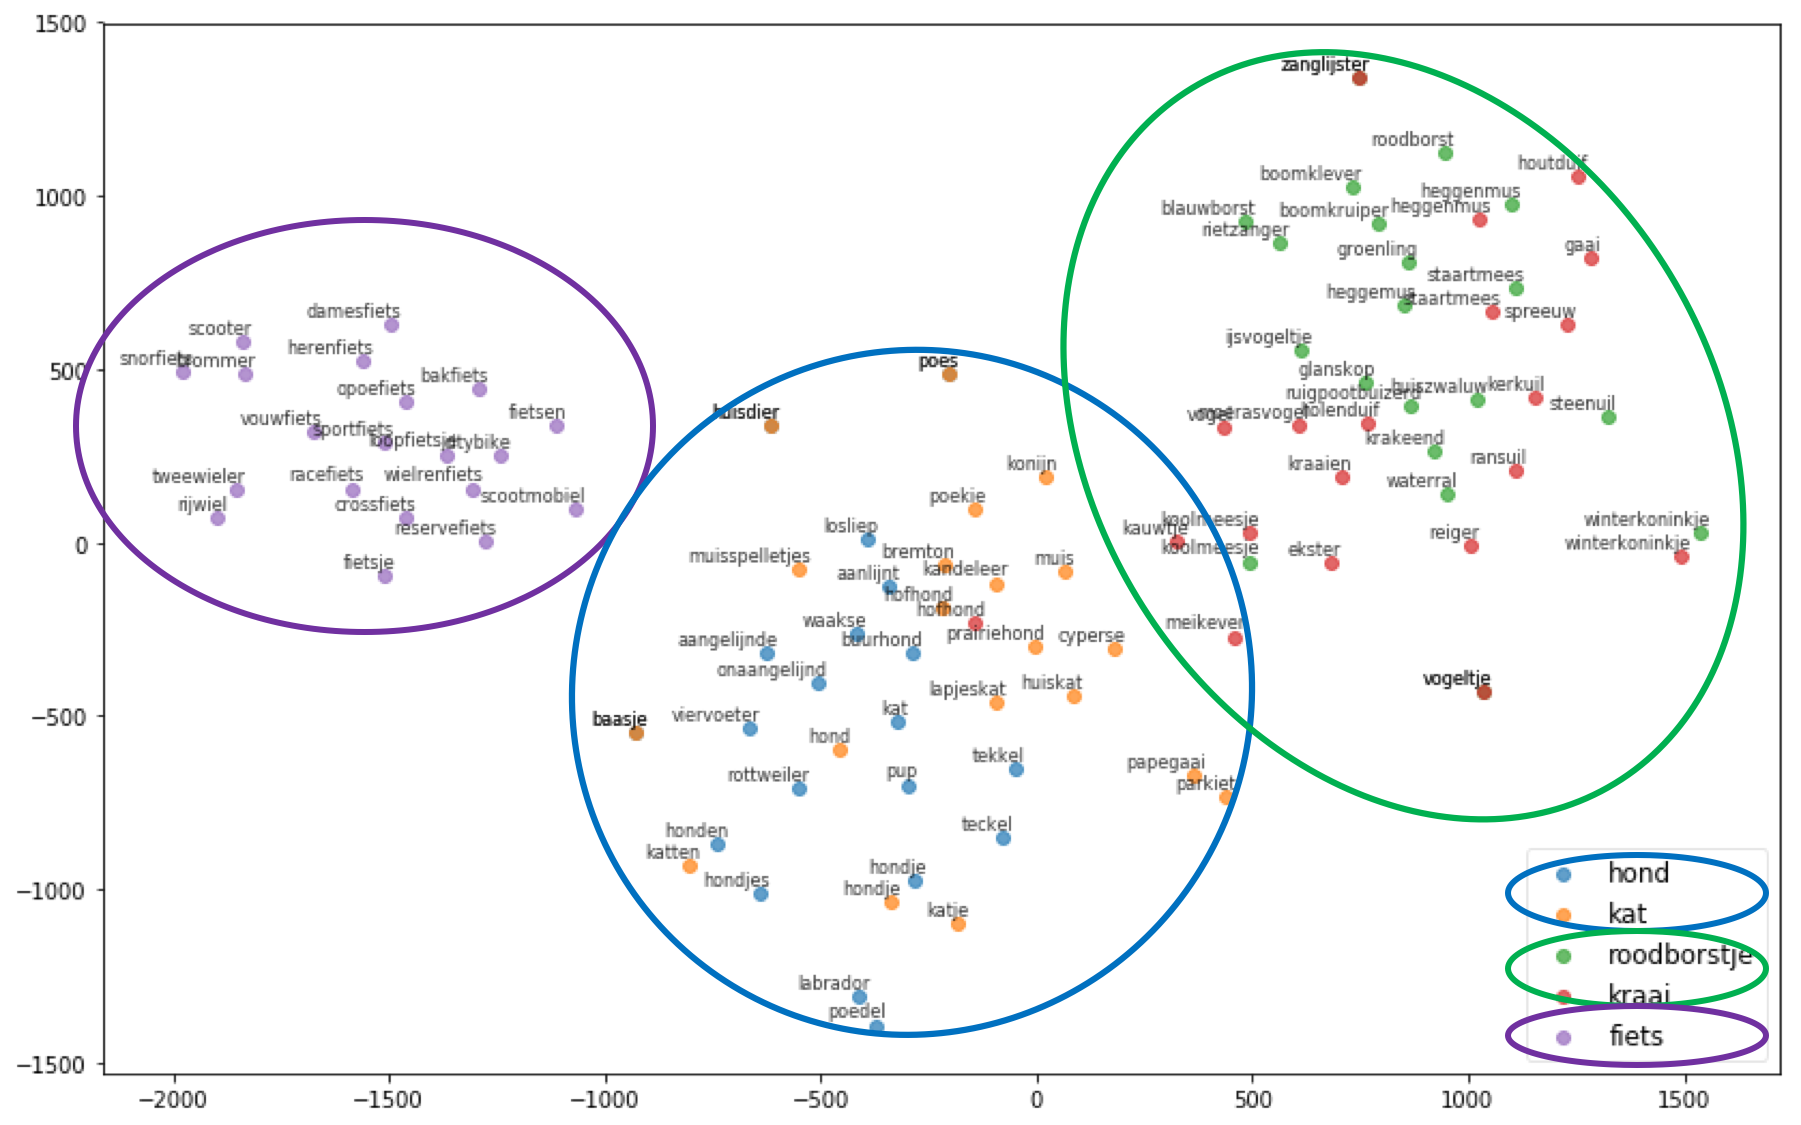
\includegraphics[width=\linewidth,height=0.6\textheight,keepaspectratio]{visual.png}}
    \begin{itemize}
        \item \href{https://projector.tensorflow.org/}{TensorFlow Projector --- explore word embeddings in 3D}
    \end{itemize}
\end{frame}

\begin{frame}{Why use pretrained embeddings?}
    Training embeddings from scratch requires \textbf{massive amounts of text} and computing power.

    \vspace{0.5em}
    \textbf{Pretrained models} are trained once on large corpora and shared openly:

    \vspace{0.5em}
    \begin{columns}
        \column{0.5\textwidth}
        \begin{itemize}
            \item \textbf{Word2Vec} (Google News)
            \item \textbf{GloVe} (Common Crawl)
        \end{itemize}
        \column{0.5\textwidth}
        \begin{itemize}
            \item \textbf{fastText} (subword info)
            \item \textbf{BERT} (contextualized)
        \end{itemize}
    \end{columns}

    \vspace{0.5em}
    \small \textbf{Note:} Word2Vec and GloVe give each word \emph{one fixed vector}. BERT gives a word a \emph{different vector depending on its context} --- \texttt{"bank"} in \emph{"river bank"} vs.\ \emph{"bank account"} gets different vectors. We will return to this later.
\end{frame}

\begin{frame}{Embeddings in communication science}
    \textbf{What can we do with embeddings that we could not do before?}
    \begin{itemize}
        \item \textbf{Sentiment analysis:} understand audience reactions beyond keyword matching
        \item \textbf{Recommender systems:} suggest content based on semantic similarity 
        \item \textbf{Text similarity:} measure how alike two texts are in meaning
    \end{itemize}

    \vspace{0.3em}
    \textbf{Note:} we will work with embeddings hands-on next week.
\end{frame}

\begin{frame}{Embeddings in practice: spaCy}
    \href{https://github.com/uva-cw-ccs2/2425s2/blob/main/week02/exercise-lecture/visualize-embeddings.ipynb}{Notebook: If you want to visualize your own embeddings}
    \begin{center}
        
\includegraphics[width=0.8\linewidth]{vectors.png}
    \end{center}
\end{frame}

% ================================
\section*{Wrap-up}
% ================================

\begin{frame}{Key takeaways}
    \begin{itemize}
        \item \textbf{Preprocessing} shapes what your model sees --- choices matter
        \item \textbf{Vectorizers} turn text into numerical matrices of token counts
        \item \textbf{TF-IDF} improves on raw counts by downweighting common tokens
        \item \textbf{Pruning} removes very rare or very frequent tokens
        \item \textbf{Bag-of-words ignores meaning} --- synonyms and related words are unrelated features
        \item \textbf{Word embeddings} capture meaning and context by learning from large corpora
        \item There is no single best approach --- it depends on your data and question
    \end{itemize}
\end{frame}

\begin{frame}{Next week}
    \begin{itemize}
        \item Text similarity and distance measures
        \item Building a simple content-based recommender system
        \item Using embeddings for document comparison
    \end{itemize}
\end{frame}

\begin{frame}{Thank you!}
    \begin{block}{Questions or comments?}
        \begin{itemize}
            \item \textbar\ a.c.kroon@uva.nl 
        \end{itemize}
    \end{block}
\end{frame}

\begin{frame}[t,allowframebreaks]
    \frametitle{References}
    \printbibliography
\end{frame}

\end{document}
